% =====================================================================
%  TELFOR 2026 -- Telekomunikacioni forum, Beograd
%  Rad: Completus: QLoRA fine-tuning modela za kod od 1,5 milijardi
%       parametara na potrošačkom GPU-u za lokalnu autokompletaciju
%  Autori: Nejra Smajlović (Univerzitet u Zenici, Politehnički fakultet)
%          Adi Kadušić     (Univerzitet u Zenici, Politehnički fakultet)
%          Alen Begović    (Univerzitet u Sarajevu, Elektrotehnički fakultet)
%
%  BOSANSKA VERZIJA rada telfor2026_completus.tex. Sadržaj, brojke i
%  zaključci su identični; razlikuje se samo jezik i decimalni zarez.
%
%  USKLAĐENOST S TELFOR PRAVILIMA:
%    * dvokolonski A4, standardni IEEE konferencijski template (IEEEtran, 10 pt)
%    * najviše 4 stranice A4 za redovne i studentske radove
%
%  Slika:  python3 Telfor2026/make_figures_completus.py
%  Build:  pdflatex telfor2026_completus_bs.tex   (pokrenuti dva puta)
% =====================================================================
\documentclass[10pt,conference,a4paper]{IEEEtran}
\IEEEoverridecommandlockouts

\usepackage[T1]{fontenc}
\usepackage[utf8]{inputenc}
\usepackage[croatian]{babel}   % prelamanje riječi; bosanski nema zaseban obrazac
\usepackage{cite}
\usepackage{graphicx}
\usepackage{amsmath}
\usepackage{booktabs}
\usepackage{balance}
\usepackage{url}
\usepackage[hidelinks]{hyperref}
\usepackage{upgreek}   % uspravna grčka slova: IEEE ne kurzivira grčke simbole

% --- Nazivi elemenata na bosanskom -----------------------------------
% babel učitava svoje natpise tek u \begin{document}, pa preambula ne vrijedi;
% umeću se u babelov popis natpisa za hrvatski.
\addto\captionscroatian{%
  \renewcommand{\abstractname}{Sažetak}%
  \renewcommand{\IEEEkeywordsname}{Ključne riječi}%
  \renewcommand{\refname}{Literatura}%
  \renewcommand{\figurename}{Slika}%
  \renewcommand{\tablename}{Tabela}%
}

% --- Tipografija tabela ----------------------------------------------
\newcommand{\best}[1]{\textbf{#1}}

% --- Copyright napomena na dnu prve stranice -------------------------
% TELFOR u uputstvu za autore ne traži IEEE copyright liniju na radu koji se
% predaje, a nema je ni zvanični IEEE konferencijski template, pa se rad
% predaje bez nje umjesto s rezerviranim mjestom.
%\IEEEpubid{\parbox{\columnwidth}{\footnotesize
%  978-1-XXXX-XXXX-X/26/\$31.00~\copyright2026 IEEE\hfill}
%  \hspace{\columnsep}\makebox[\columnwidth]{}}

\begin{document}

\title{Completus: QLoRA fine-tuning modela za kod od\\
1,5 milijardi parametara na potrošačkom GPU-u}

\author{\IEEEauthorblockN{Nejra Smajlović}
\IEEEauthorblockA{\textit{Univerzitet u Zenici}\\
\textit{Politehnički fakultet}\\
Zenica, Bosna i Hercegovina\\
nejra.smajlovic.22@size.ba}
\and
\IEEEauthorblockN{Adi Kadušić}
\IEEEauthorblockA{\textit{Univerzitet u Zenici}\\
\textit{Politehnički fakultet}\\
Zenica, Bosna i Hercegovina\\
adi.kadusic.22@size.ba}
\and
\IEEEauthorblockN{Alen Begović}
\IEEEauthorblockA{\textit{Univerzitet u Sarajevu}\\
\textit{Elektrotehnički fakultet}\\
Sarajevo, Bosna i Hercegovina\\
alen.begovic@etf.unsa.ba}%
\thanks{N. Smajlović i A. Kadušić su s Politehničkog fakulteta Univerziteta u
Zenici, a A. Begović s Elektrotehničkog fakulteta Univerziteta u Sarajevu,
Bosna i Hercegovina. Kod za treniranje, Modelfile datoteke i skripte za
evaluaciju: \url{https://github.com/kadusic1/completus}.}}

\maketitle
\bstctlcite{bstctl:completus}

\begin{abstract}
Ovaj rad predstavlja Completus, reproducibilan pipeline koji specijalizuje
otvoreni model za kod od 1,5 milijardi parametara za lokalnu autokompletaciju
bez mrežnog pristupa, na jednoj potrošačkoj grafičkoj kartici.
Qwen2.5-Coder-1.5B se fino podešava QLoRA adapterom fiksnog ranga nad
kuriranim Python i Go podskupovima CodeSearchNeta, nakon faze pripreme koja
spaja uklanjanje bliskih duplikata, filtriranje mirisa koda, provjeru
kvaliteta dokumentacijskih nizova i fill-in-the-middle transformaciju.
Istrenirani adapter se spaja u osnovne težine, izvozi u četverobitni
K-kvantizovani GGUF oblik i servira kroz Ollamu, čime model postaje dostupan
standardnom dodatku za editor bez ijednog mrežnog poziva. Pri evaluaciji na
HumanEvalu, uz protokol vjeran načinu isporuke u kojem je upit goli potpis
funkcije, fino podešeni Python model rješava 42,68 posto problema iz prvog
pokušaja, naspram 10,98 posto koliko postiže nepodešena osnovna verzija pod
istim protokolom. Dobitak je stoga oporavak sposobnosti koju osnovni model
već prijavljuje pod vlastitim, povoljnijim protokolom, ostvaren u formatu
upita koji lokalna isporuka zaista koristi, a ne neto prirast sposobnosti.
Cijeli tok izvršava se na laptop grafičkoj kartici od osam gigabajta za manje
od dva sata po jeziku.
\end{abstract}

\begin{IEEEkeywords}
autokompletacija koda, QLoRA, parametarski efikasno fino podešavanje,
Qwen2.5-Coder, CodeSearchNet, GGUF kvantizacija, lokalna inferencija.
\end{IEEEkeywords}

% =====================================================================
\section{Uvod}
% =====================================================================
\IEEEPARstart{V}{eliki} jezički modeli (LLM) specijalizovani za kod daju
tačnu autokompletaciju i svijest o kontekstu kroz više datoteka, ali
komercijalni sistemi koji vode po tim mjerama dostupni su isključivo preko
cloud servisa. Takav način isporuke nosi tri troška koja su neprihvatljiva u
reguliranim djelatnostima, u okruženjima odsječenim od mreže i u budžetski
ograničenim timovima: stalnu mrežnu vezu, izlaganje vlasničkog izvornog koda
infrastrukturi treće strane i naplatu po tokenu koja nikad ne prestaje. Model
dovoljno mali da radi na radnoj stanici samog programera, na jednoj
potrošačkoj grafičkoj procesorskoj jedinici (GPU), uklanja sva tri odjednom.

Lokalna isporuka uvodi drugo ograničenje. Model mora biti dovoljno kompaktan
da odgovori unutar vremenskog budžeta dodatka za editor na uobičajenom
hardveru, a opet dovoljno sposoban da njegove dopune vrijedi prihvatiti. Dva
razvoja čine taj kompromis izvodljivim. Parametarski efikasno fino
podešavanje (PEFT), posebno adaptacija niskog ranga
(LoRA)~\cite{hu2022lora}, specijalizuje prethodno istrenirani model uz mali
dio troška potpunog podešavanja; kvantizovani formati težina poput GGUF-a,
servirani optimizovanim izvršnim okruženjima, izvršavaju te težine unutar
nekoliko gigabajta video memorije.

Ovaj rad iznosi cjelovitu realizaciju tog recepta, nazvanu Completus, i
evaluira je u uslovima u kojima se zaista servira. Dvije praznine motivišu
rad. Prvo, objavljene studije iznose ili sirovu sposobnost modela ili
tehniku adaptacije, izolovano; malo ih vodi jedan model od sirovog korpusa
kroz kuriranje podataka, adaptaciju i kvantizaciju do žive tačke pristupa
integrisane u editor, uz izvještaj o svakoj fazi. Drugo, modeli za kod
obično se ocjenjuju pod few-shot protokolima u formatu razgovora, koji ne
liče na gole potpise funkcija kakve šalje dodatak za editor, pa objavljena
ocjena ne predviđa ono što će programer doživjeti. Doprinosi rada su
cjelovit pipeline sa Slike~\ref{fig:pipeline}, iznesen s parametrima
potrebnim za reprodukciju; kvantifikacija efekta jedne QLoRA epohe izmjerena
u formatu upita kakav isporuka koristi; i izričito razdvajanje oporavka
sposobnosti od prirasta sposobnosti, što određuje protokol evaluacije, a što
objavljene ocjene redovno miješaju.

\begin{figure*}[!t]
\centering
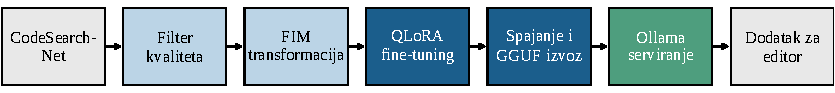
\includegraphics[width=\textwidth]{figures/fig_pipeline_bs.pdf}
\caption{Completus pipeline. Sirove CodeSearchNet funkcije prolaze kroz
filtriranje kvaliteta i fill-in-the-middle transformaciju, specijalizuju
Qwen2.5-Coder-1.5B kroz QLoRA, te se spajaju i izvoze u četverobitni
K-kvantizovani GGUF oblik koji Ollama servira dodatku za editor preko lokalne
loopback petlje.}
\label{fig:pipeline}
\end{figure*}

% =====================================================================
\section{Dosadašnja istraživanja}
% =====================================================================
Oslanjajući se na Transformer arhitekturu s isključivo dekoderskim
slojevima~\cite{vaswani2017}, niz otvorenih modela za kod smanjio je zaostatak
za vlasničkim sistemima. StarCoder~\cite{li2023starcoder} trenira se nad
permisivno licenciranim Stack korpusom uz multi-query attention i
fill-in-the-middle (FIM) cilj; Code Llama~\cite{roziere2023} proširuje
Llamu~2 popunjavanjem i podrškom za dug kontekst;
DeepSeek-Coder~\cite{guo2024} trenira se nad korpusom na nivou projekta uz
cilj popunjavanja; a Qwen2.5-Coder~\cite{hui2024} prijavljuje vodeće rezultate
među otvorenim modelima na skali od 1,5 milijardi parametara koja se ovdje
koristi. Completus se razlikuje po cilju, a ne po tehnici: ne trenira novi
model, nego specijalizuje postojeći mali za uzak zadatak osjetljiv na
kašnjenje.

Na strani adaptacije, LoRA~\cite{hu2022lora} zamrzava prethodno istrenirane
težine i ubacuje matrice niskorangovane dekompozicije, smanjujući broj
parametara koji se treniraju za nekoliko redova veličine. Kvantizovana LoRA
(QLoRA)~\cite{dettmers2023} kvantizuje zamrznutu bazu na četverobitni
NormalFloat (NF4), čime fino podešavanje ulazi u memorijski budžet jedne
potrošačke kartice. AdaLoRA~\cite{zhang2023adalora} razrađuje raspodjelu ranga
prema važnosti. Weyssow i drugi~\cite{weyssow2025} evaluiraju PEFT konkretno
za generisanje koda i potvrđuju da LoRA vraća najveći dio kvaliteta potpunog
podešavanja uz dio njegove cijene, a pregled Hana i drugih~\cite{han2024}
smješta LoRA-u u širu PEFT porodicu.

Treća linija tiče se podataka za treniranje. Xue i drugi~\cite{xue2025}
pokazuju da uklanjanje mirisa koda poboljšava kvalitet modela; Lee i
drugi~\cite{lee2022} da uklanjanje bliskih duplikata smanjuje memorisanje i
curenje testnog materijala; Bavarian i drugi~\cite{bavarian2022} da modeli
stiču sposobnost popunjavanja bez gubitka u generisanju slijeva nadesno; a
WizardCoder~\cite{luo2024} da podešavanje u stilu instrukcija dalje podiže
kvalitet koda. Izbor kvantizacije slijedi objedinjenu evaluaciju llama.cpp
formata koju daje Kurt~\cite{kurt2026}. Ovim radovima zajedničko je to da je svaki razvijen
i prikazan u istraživačkom ili cloud okruženju, pod protokolom koji su
odabrali njihovi autori. Nijedan ne daje recept koji mali otvoreni model vodi
sve do tačke pristupa integrisane u editor na uobičajenom hardveru, uz
izvještaj o kvalitetu u formatu upita koji ta tačka prima.

% =====================================================================
\section{Completus pipeline}
% =====================================================================
Pipeline ima pet faza, prikazanih na Slici~\ref{fig:pipeline}: priprema
podataka, QLoRA fino podešavanje, spajanje adaptera, GGUF izvoz i lokalna
registracija za serviranje. Svaka faza je skriptovana i parametrizovana, tako
da se cijeli put od javnog korpusa do žive tačke pristupa može ponovo izvesti
na jednoj mašini.

\subsection{Priprema podataka}
Korpus je CodeSearchNet~\cite{husain2019}, čiji puni podskupovi sadrže
412\,178 Python i 317\,832 Go funkcija. Da bi priprema ostala izvodljiva na
jednoj radnoj stanici, ulaz je ograničen na prvih 50\,000 funkcija po jeziku,
koje zatim prolaze kroz pet filtera. Bliski duplikati uklanjaju se heširanjem
osjetljivim na lokalnost nad MinHash sažecima (128 permutacija, šindre od pet
tokena, Jaccardov prag 0,8). Filter mirisa koda odbacuje linije duže od 120
znakova, funkcije kraće od 30 tokena i tijela koja ništa ne rade. Filter
dokumentacijskih nizova traži najmanje 15 tokena i dvije riječi i odbija
svaki niz koji nosi oznaku TODO, FIXME ili XXX. Fill-in-the-middle
transformacija zatim se primjenjuje na 80~\% preživjelih uzoraka, a ostatak
se skraćuje na 2048 tokena.

Svaki filter cilja dokumentovani način otkaza, a ne opštu urednost. Uklanjanje
bliskih duplikata primjenjuje se jer dupliran tekst za treniranje povećava
memorisanje i propušta testni materijal u treniranje~\cite{lee2022}; filter
mirisa koda jer modeli trenirani nad očišćenim korpusima daju bolji
kod~\cite{xue2025}; a FIM transformacija jer donosi sposobnost popunjavanja,
koja je ono što dodatak za editor treba, bez izmjerenog gubitka u generisanju
slijeva nadesno~\cite{bavarian2022}.

Tabela~\ref{tab:data} prikazuje šta preživi. Zadržavanje se oštro razlikuje
između dva jezika, 63,9~\% za Python naspram 42,6~\% za Go, a jaz je
dominantno posljedica filtera dokumentacijskih nizova, jer su idiomatski Go
komentari često kraći od praga od 15 tokena. Posljedica je da dva adaptera
nisu trenirana nad usporedivom količinom podataka, što se mora imati u vidu
pri poređenju dva modela.

\begin{table}[b]
\caption{Podaci za treniranje koji preživljavaju pripremni pipeline}
\label{tab:data}
\centering
\footnotesize
\begin{tabular}{@{}lrrr@{}}
\toprule
\textbf{Jezik} & \textbf{Ulazni prag} & \textbf{Nakon pipelinea} & \textbf{Zadržano}\\
\midrule
Python & 50\,000  & 31\,966 & 63,9~\%\\
Go     & 50\,000  & 21\,284 & 42,6~\%\\
\midrule
Ukupno & 100\,000 & 53\,250 & 53,3~\%\\
\bottomrule
\end{tabular}
\end{table}

\subsection{QLoRA fino podešavanje}
Qwen2.5-Coder-1.5B~\cite{hui2024} učitava se u četverobitnoj NF4 kvantizaciji
i adaptira QLoRA-om~\cite{dettmers2023} kroz Unsloth izvršno okruženje.
Adapteri se kače na svih sedam linearnih projekcijskih matrica, pri fiksnom
rangu umjesto adaptivno raspoređenog, tako da je memorijski plafon poznat
unaprijed na kartici od osam gigabajta. Tabela~\ref{tab:config} navodi
cjelovitu konfiguraciju.

\begin{table}[b]
\caption{Konfiguracija QLoRA finog podešavanja}
\label{tab:config}
\centering
\footnotesize
\begin{tabular}{@{}ll@{}}
\toprule
\textbf{Parametar} & \textbf{Vrijednost}\\
\midrule
Osnovni model             & Qwen2.5-Coder-1.5B\\
Kvantizacija              & četverobitni NF4\\
LoRA rang / skaliranje    & 16 / 32\\
Ciljni moduli             & q, k, v, o, gate, up, down\\
Veličina serije / akumulacija & 2 / 8 (efektivno 16)\\
Stopa učenja / raspored   & 0,0002 / kosinusni\\
Optimizator               & AdamW, osmobitni\\
Epohe / maks.\ dužina niza & 1 / 2048\\
Nasumično sjeme           & 3407\\
Hardver                   & NVIDIA RTX 4060 Laptop (8\,GB)\\
\bottomrule
\end{tabular}
\end{table}

Budžet od osam gigabajta je ono što diktira tu konfiguraciju. Fino
podešavanje svih parametara modela ove veličine u mješovitoj preciznosti
traži oko 16 bajtova po parametru kada su prisutne poluprecizne težine,
njihovi gradijenti, jednoprecizna master kopija i oba AdamW momenta, što je
otprilike 24\,GB, ili tri puta više nego što kartica nudi. QLoRA gotovo sve
to uklanja: zamrznuta baza u četverobitnom NF4 zauzima ispod jednog
gigabajta, a pošto se treniraju samo ubačene niskorangovane matrice,
gradijenti i stanje optimizatora postoje za mali dio parametara, prepolovljeni
još jednom osmobitnim optimizatorom. Ono što ostaje od budžeta troši se na
aktivacije, čiji vrhunac određuju dužina niza od 2048 tokena i veličina
mikro-serije. Zato je serija podijeljena na dva uzorka s osmostrukom
akumulacijom gradijenta umjesto šesnaest odjednom: podjela ostavlja efektivnu
veličinu serije nepromijenjenom, a vrhunac aktivacija zadržava unutar
kartice, i to je postavka koja odlučuje hoće li izvođenje uopšte stati.

Svaki jezik trenira se jednu epohu: 1998 koraka optimizatora za Python i 1331
za Go, pri efektivnoj veličini serije od 16. Go izvođenje završilo je za
3713~s (62~min), a Python za približno 2,2~h, pa cijeli jezik staje unutar
jedne radne sesije na laptopu. Gubitak pri treniranju pada s 1,674 na početku
Python izvođenja, a Go izvođenje završava sa srednjim gubitkom od 1,111.

\subsection{Spajanje, izvoz i lokalno serviranje}
Nakon treniranja, LoRA težine spajaju se u osnovni checkpoint i izvoze kao
kvantizovani GGUF binarni fajl u \texttt{q4\_k\_m} shemi, koju objedinjena
evaluacija llama.cpp formata~\cite{kurt2026} prepoznaje kao povoljan
kompromis između veličine i kvaliteta, mada ta evaluacija pokriva model od
osam milijardi parametara, pa se njeni zaključci na manji prenose
neprovjereno. K-kvant sheme nisu uniformni četverobitni formati:
\texttt{q4\_k\_m} zadržava dio attention i feed-forward projekcija na šest
bita, a ostatak zaokružuje na četiri, trošeći dodatne bitove tamo gdje je
cijena zaokruživanja po tačnost najveća. Ta neuniformnost, a ne nominalna
širina u bitovima, čini je uobičajenim izborom na ovom nivou kvantizacije.

Svaki binarni fajl registruje se s Ollamom kroz Modelfile koji fiksira FIM
predložak upita, temperaturu dekodiranja 0, kontekstni prozor od 2048 tokena i
granicu generisanja od 256 tokena. Rezultat je tačka pristupa na lokalnoj
loopback petlji, koju direktno koristi Continue.dev dodatak za editor; nijedan
zahtjev ne napušta mašinu.

\subsection{Hardverska ograničenja lokalnog serviranja}
Kvantizacija je bitna i za serviranje, ne samo da bi model stao, a razlog leži
u uređaju, a ne u modelu. Autoregresivno dekodiranje pri seriji od jednog
uzorka svodi svako množenje matricom na proizvod matrice i vektora, u kojem
se svaka težina pročita jednom i jednom upotrijebi. Ne preostaje ponovna
upotreba koju bi tenzorske jedinice iskoristile, pa aritmetički intenzitet
pada na oko jedne operacije po bajtu, a brzinu dekodiranja određuje propusnost
memorije, a ne računska propusnost.

Plafon je zato unaprijed izračunljiv. Korištena kartica spaja 8\,GB GDDR6
memorije sa 128-bitnom magistralom pri 16\,Gbit/s po pinu, što daje
256\,GB/s. \texttt{q4\_k\_m} izdanje modela od 1,54 milijarde parametara
zauzima oko 1\,GB, pa se i uz potpuno zasićen memorijski podsistem može
proizvesti najviše oko 250 tokena u sekundi; spojeni poluprecizni checkpoint
zauzima 3,1\,GB i ograničen je na oko 80. Faktor tri između njih posljedica je
propusnosti, a ne manjeg broja izvršenih operacija.

Dva člana korigiraju tu granicu u suprotnim smjerovima. Keš ključeva i
vrijednosti čita se uz težine, oko 28\,kB po tokenu za ovu arhitekturu, pa
pun prozor od 2048 tokena dodaje oko 60\,MB po koraku, ispod desetine
saobraćaja težina. Nasuprot tome, K-kvantizovani blokovi moraju se raspakovati
prije množenja, trošeći račun koji poluprecizni put ne troši, pa je ostvareno
ubrzanje manje nego što omjer saobraćaja sugeriše. Prefill se opet ponaša
drugačije: prompt se obrađuje u jednom prolazu, čime se vraća ponovna
upotreba i ta faza postaje računski ograničena, pa vrijeme do prvog prijedloga
i razmak između tokena ograničavaju različiti dijelovi uređaja.

Sve navedeno su granice izvedene iz objavljenih parametara uređaja i modela, a
ne mjerenja; odjeljak~\ref{sec:limits} bilježi da ostvarene vrijednosti nisu
prikupljene.

% =====================================================================
\section{Evaluacija}
% =====================================================================
\subsection{Protokol}
Evaluacija koristi HumanEval, čijih 164 Python problema svaki uparuje potpis
funkcije sa skrivenim jediničnim testovima. Generisanje je pohlepno, jedan
determinističan uzorak po problemu i najviše 512 novih tokena, a prikazana
metrika je pass@1: udio problema čije generisano tijelo prolazi sve testove.

Prikazuje se samo pass@1. Brojanje problema riješenim ako prođe bilo koja od
više uzorkovanih dopuna mjeri svojstvo koje nijedan dodatak za editor ne
izlaže: programer vidi jedan prijedlog i prihvata ga ili ne. Pohlepni pass@1
stoga mjeri ono što isporuka daje, po cijenu šireg intervala povjerenja.

Format upita ovdje je važniji od dekodiranja. Umjesto few-shot upita u formatu
razgovora, kakav koristi izvještaj samog osnovnog modela, upit je goli potpis
funkcije, što je ono što dodatak za editor šalje. Oba checkpointa evaluiraju
se pod istovjetnim uslovima, pa je poređenje između njih interno valjano iako
nijedan broj nije uporediv s objavljenom ocjenom dobijenom pod drugačijim
protokolom. Pošto je dekodiranje determinističko, jedini izvor nesigurnosti
je konačan skup problema, pa se prikazuju 95~\% Wilsonovi intervali
povjerenja (CI).

\subsection{Rezultati}
Fino podešeni Python model rješava 70 od 164 problema, što je pass@1 od
42,68~\% uz 95~\% interval povjerenja [35,4, 50,3]. Nepodešena osnovna
verzija rješava 18, što je pass@1 od 10,98~\% uz interval [7,1, 16,7].
Intervali se ne preklapaju, pa je razlika od 31,7 procentnih poena
razlučiva od šuma uzorkovanja pod ovim protokolom.

\subsection{Čitanje rezultata naspram objavljenih ocjena}
Tumačenje te razlike u potpunosti ovisi o tome šta mjeri broj osnovne
verzije. Pod vlastitim few-shot protokolom, isti osnovni model prijavljen je
na 43,9~\%~\cite{hui2024} --- gotovo tačno ono što fino podešeni model ovdje
dostiže. Osnovnih 10,98~\% stoga ne opisuje slab model; opisuje sposoban
model kažnjen formatom upita za koji nije bio pripremljen. Jedna QLoRA epoha
uči ga da tijelo funkcije generiše direktno iz potpisa, čime se ta latentna
sposobnost vraća u formatu koji isporuka koristi. Tabela~\ref{tab:humaneval}
stavlja oba broja uz objavljene ocjene za usporedive modele; te ocjene
dobijene su pod protokolima koje su odredili njihovi autori i predstavljaju
kontekst, a ne kontrolisano poređenje.

\begin{table}[b]
\caption{HumanEval pass@1. Gornji blok mjeren je ovdje pod jednim protokolom;
donji blok prenosi objavljene ocjene dobijene pod protokolima koji se
razlikuju od njega i međusobno}
\label{tab:humaneval}
\centering
\footnotesize
\begin{tabular}{@{}llrl@{}}
\toprule
\textbf{Model} & \textbf{Parametri} & \textbf{pass@1} & \textbf{95~\% CI}\\
\midrule
\multicolumn{4}{@{}l}{\emph{Mjereno ovdje, protokol s golim potpisom}}\\
Qwen2.5-Coder-1.5B (osnovni) & 1,5B & 10,98~\% & [7,1, 16,7]\\
Completus Python (podešeni) & 1,5B & \best{42,68~\%} & [35,4, 50,3]\\
\midrule
\multicolumn{4}{@{}l}{\emph{Objavljeno, svaki pod vlastitim protokolom}}\\
CodeLlama-Base~\cite{guo2024}       & 7B    & 31,7~\% & ---\\
StarCoderBase~\cite{guo2024}        & 15,5B & 31,7~\% & ---\\
DeepSeek-Coder-Base~\cite{guo2024}  & 1,3B  & 34,8~\% & ---\\
Qwen2.5-Coder osnovni~\cite{hui2024} & 1,5B & 43,9~\% & ---\\
\bottomrule
\end{tabular}
\end{table}

% =====================================================================
\section{Diskusija i ograničenja validnosti}
\label{sec:limits}
% =====================================================================
Praktično čitanje jeste da kompaktan otvoren model, adaptiran dva sata na
laptop kartici, servira autokompletaciju kvaliteta bliskog onome što
prijavljuju njegovi autori, bez mrežne ovisnosti i bez troška po tokenu. Ono
što fino podešavanje donosi nije inteligencija nego usklađivanje formata, i ta
razlika je glavna metodološka poenta rada: ocjena na benchmarku je zajedničko
svojstvo modela i protokola upita, pa se ocjena dobijena pod povoljnim
protokolom ne prenosi na isporuku koja pita drugačije. To je u skladu s
nalazom Weyssowa i drugih~\cite{weyssow2025} da LoRA vraća najveći dio
kvaliteta potpunog podešavanja, i govori u prilog evaluaciji pod protokolom
koji će sistem zaista primati.

Za tim koji vaga hostovanu naspram lokalne tačke pristupa, cijena odlaska u
lokalno je jedna kartica laptop klase i dva sata treniranja po jeziku.
Poređenje u Tabeli~\ref{tab:humaneval} pokazuje i da veličina modela nije
cijela priča na ovoj skali: adaptirani model od 1,5 milijardi
parametara dostiže ocjenu usporedivu s objavljenim brojevima za modele četiri
do deset puta veće, mada pod protokolima koji se razlikuju, pa samo kao
naznaka.

Pet ograničenja omeđuje ove rezultate. Prvo, samo je Python model evaluiran
kvantitativno; Go model ocijenjen je kvalitativno, pa jaz u zadržavanju iz
odjeljka~III-A nije vezan za izmjerenu razliku u kvalitetu. Drugo, HumanEval
ocjenjuje sintezu samostalnih funkcija, a ne popunjavanje svjesno položaja
kursora, koje FIM cilj trenira i koje dodatak za editor zaista traži, pa
prikazani broj ne mjeri isporučeni zadatak direktno. Treće, ulaz u pipeline
ograničen je na 50\,000 funkcija po jeziku, a pragovi filtera su fiksni, pa su
stope zadržavanja jedna radna tačka, a ne podešeni optimum. Četvrto, po jednom
jeziku izvedeno je jedno treniranje uz fiksno sjeme, pa varijansa između
izvođenja nije kvantifikovana. Peto, i najvažnije za navedenu motivaciju,
isporučeni artefakt je analitički omeđen u odjeljku~III-D, ali nikad izmjeren:
nisu prikazani ni kašnjenje dopune, ni propusnost, ni zauzeće memorije pri
inferenciji, a efekat četverobitne kvantizacije na kvalitet odgovora nije
odvojen od efekta finog podešavanja.

% =====================================================================
\section{Zaključak}
% =====================================================================
Completus vodi otvoreni model za kod od 1,5 milijardi parametara od javnog
korpusa do tačke pristupa integrisane u editor koja radi u cijelosti na
potrošačkoj kartici od osam gigabajta, i izvještava o svakoj fazi tog puta.
Jedna QLoRA epoha podiže HumanEval pass@1 s 10,98~\% na 42,68~\% pod
protokolom s golim potpisom, približavajući se vrijednosti od 43,9~\% koju
osnovni model prijavljuje pod vlastitim, povoljnijim protokolom. Taj rezultat
najbolje je čitati kao oporavak, a ne kao prirast: fino podešavanje usklađuje
model s formatom upita koji isporuka šalje, a veličina efekta mjeri koliko
neusklađenost protokola može prigušiti inače sposoban model. Buduća istraživanja
izmjerit će servisiranu tačku pristupa naspram granica iz odjeljka~III-D,
evaluirati Go model na HumanEval-X i uvesti benchmark svjestan popunjavanja
koji odgovara isporučenoj upotrebi.

\section*{Zahvala}
Rad je nastao kao projekat iz predmeta Optimizacija baza podataka na
Politehničkom fakultetu Univerziteta u Zenici.

\balance

% =====================================================================
\bibliographystyle{IEEEtran}
\bibliography{refs_completus}

\end{document}
